% Options for packages loaded elsewhere
\PassOptionsToPackage{unicode}{hyperref}
\PassOptionsToPackage{hyphens}{url}
%
\documentclass[
]{book}
\usepackage{amsmath,amssymb}
\usepackage{iftex}
\ifPDFTeX
  \usepackage[T1]{fontenc}
  \usepackage[utf8]{inputenc}
  \usepackage{textcomp} % provide euro and other symbols
\else % if luatex or xetex
  \usepackage{unicode-math} % this also loads fontspec
  \defaultfontfeatures{Scale=MatchLowercase}
  \defaultfontfeatures[\rmfamily]{Ligatures=TeX,Scale=1}
\fi
\usepackage{lmodern}
\ifPDFTeX\else
  % xetex/luatex font selection
\fi
% Use upquote if available, for straight quotes in verbatim environments
\IfFileExists{upquote.sty}{\usepackage{upquote}}{}
\IfFileExists{microtype.sty}{% use microtype if available
  \usepackage[]{microtype}
  \UseMicrotypeSet[protrusion]{basicmath} % disable protrusion for tt fonts
}{}
\makeatletter
\@ifundefined{KOMAClassName}{% if non-KOMA class
  \IfFileExists{parskip.sty}{%
    \usepackage{parskip}
  }{% else
    \setlength{\parindent}{0pt}
    \setlength{\parskip}{6pt plus 2pt minus 1pt}}
}{% if KOMA class
  \KOMAoptions{parskip=half}}
\makeatother
\usepackage{xcolor}
\usepackage{color}
\usepackage{fancyvrb}
\newcommand{\VerbBar}{|}
\newcommand{\VERB}{\Verb[commandchars=\\\{\}]}
\DefineVerbatimEnvironment{Highlighting}{Verbatim}{commandchars=\\\{\}}
% Add ',fontsize=\small' for more characters per line
\usepackage{framed}
\definecolor{shadecolor}{RGB}{248,248,248}
\newenvironment{Shaded}{\begin{snugshade}}{\end{snugshade}}
\newcommand{\AlertTok}[1]{\textcolor[rgb]{0.94,0.16,0.16}{#1}}
\newcommand{\AnnotationTok}[1]{\textcolor[rgb]{0.56,0.35,0.01}{\textbf{\textit{#1}}}}
\newcommand{\AttributeTok}[1]{\textcolor[rgb]{0.13,0.29,0.53}{#1}}
\newcommand{\BaseNTok}[1]{\textcolor[rgb]{0.00,0.00,0.81}{#1}}
\newcommand{\BuiltInTok}[1]{#1}
\newcommand{\CharTok}[1]{\textcolor[rgb]{0.31,0.60,0.02}{#1}}
\newcommand{\CommentTok}[1]{\textcolor[rgb]{0.56,0.35,0.01}{\textit{#1}}}
\newcommand{\CommentVarTok}[1]{\textcolor[rgb]{0.56,0.35,0.01}{\textbf{\textit{#1}}}}
\newcommand{\ConstantTok}[1]{\textcolor[rgb]{0.56,0.35,0.01}{#1}}
\newcommand{\ControlFlowTok}[1]{\textcolor[rgb]{0.13,0.29,0.53}{\textbf{#1}}}
\newcommand{\DataTypeTok}[1]{\textcolor[rgb]{0.13,0.29,0.53}{#1}}
\newcommand{\DecValTok}[1]{\textcolor[rgb]{0.00,0.00,0.81}{#1}}
\newcommand{\DocumentationTok}[1]{\textcolor[rgb]{0.56,0.35,0.01}{\textbf{\textit{#1}}}}
\newcommand{\ErrorTok}[1]{\textcolor[rgb]{0.64,0.00,0.00}{\textbf{#1}}}
\newcommand{\ExtensionTok}[1]{#1}
\newcommand{\FloatTok}[1]{\textcolor[rgb]{0.00,0.00,0.81}{#1}}
\newcommand{\FunctionTok}[1]{\textcolor[rgb]{0.13,0.29,0.53}{\textbf{#1}}}
\newcommand{\ImportTok}[1]{#1}
\newcommand{\InformationTok}[1]{\textcolor[rgb]{0.56,0.35,0.01}{\textbf{\textit{#1}}}}
\newcommand{\KeywordTok}[1]{\textcolor[rgb]{0.13,0.29,0.53}{\textbf{#1}}}
\newcommand{\NormalTok}[1]{#1}
\newcommand{\OperatorTok}[1]{\textcolor[rgb]{0.81,0.36,0.00}{\textbf{#1}}}
\newcommand{\OtherTok}[1]{\textcolor[rgb]{0.56,0.35,0.01}{#1}}
\newcommand{\PreprocessorTok}[1]{\textcolor[rgb]{0.56,0.35,0.01}{\textit{#1}}}
\newcommand{\RegionMarkerTok}[1]{#1}
\newcommand{\SpecialCharTok}[1]{\textcolor[rgb]{0.81,0.36,0.00}{\textbf{#1}}}
\newcommand{\SpecialStringTok}[1]{\textcolor[rgb]{0.31,0.60,0.02}{#1}}
\newcommand{\StringTok}[1]{\textcolor[rgb]{0.31,0.60,0.02}{#1}}
\newcommand{\VariableTok}[1]{\textcolor[rgb]{0.00,0.00,0.00}{#1}}
\newcommand{\VerbatimStringTok}[1]{\textcolor[rgb]{0.31,0.60,0.02}{#1}}
\newcommand{\WarningTok}[1]{\textcolor[rgb]{0.56,0.35,0.01}{\textbf{\textit{#1}}}}
\usepackage{longtable,booktabs,array}
\usepackage{calc} % for calculating minipage widths
% Correct order of tables after \paragraph or \subparagraph
\usepackage{etoolbox}
\makeatletter
\patchcmd\longtable{\par}{\if@noskipsec\mbox{}\fi\par}{}{}
\makeatother
% Allow footnotes in longtable head/foot
\IfFileExists{footnotehyper.sty}{\usepackage{footnotehyper}}{\usepackage{footnote}}
\makesavenoteenv{longtable}
\usepackage{graphicx}
\makeatletter
\def\maxwidth{\ifdim\Gin@nat@width>\linewidth\linewidth\else\Gin@nat@width\fi}
\def\maxheight{\ifdim\Gin@nat@height>\textheight\textheight\else\Gin@nat@height\fi}
\makeatother
% Scale images if necessary, so that they will not overflow the page
% margins by default, and it is still possible to overwrite the defaults
% using explicit options in \includegraphics[width, height, ...]{}
\setkeys{Gin}{width=\maxwidth,height=\maxheight,keepaspectratio}
% Set default figure placement to htbp
\makeatletter
\def\fps@figure{htbp}
\makeatother
\setlength{\emergencystretch}{3em} % prevent overfull lines
\providecommand{\tightlist}{%
  \setlength{\itemsep}{0pt}\setlength{\parskip}{0pt}}
\setcounter{secnumdepth}{5}
\usepackage{booktabs}
\usepackage{ctex}
\ifLuaTeX
  \usepackage{selnolig}  % disable illegal ligatures
\fi
\usepackage[]{natbib}
\bibliographystyle{plainnat}
\IfFileExists{bookmark.sty}{\usepackage{bookmark}}{\usepackage{hyperref}}
\IfFileExists{xurl.sty}{\usepackage{xurl}}{} % add URL line breaks if available
\urlstyle{same}
\hypersetup{
  pdftitle={基于R的文献复刻:利用中国微观数据库},
  pdfauthor={黄建祺},
  hidelinks,
  pdfcreator={LaTeX via pandoc}}

\title{基于R的文献复刻:利用中国微观数据库}
\author{黄建祺}
\date{2023-03-13}

\begin{document}
\maketitle

{
\setcounter{tocdepth}{1}
\tableofcontents
}
\hypertarget{ux524dux8a00}{%
\chapter*{前言}\label{ux524dux8a00}}
\addcontentsline{toc}{chapter}{前言}

这本书是基于中国的几大微观数据库及相关的顶刊上的文章为主要内容写成的自我技术修炼笔记,为最大化他的社会效益,以 \citep{R-bookdown} 形式生成。希望能够对你有所帮助。

在经济学研究中,近些年来对于微观数据的使用变得尤为重要,尤其是大型的微观数据库的使用。但常用的处理方法往往是选择在Stata中进行操作。但在另一方面,R相对于Stata的使用有其独特的优势,尤其是在使用多个数据框操作时候,在今天的一篇文章中很难就单单一个数据源就能完成一篇好的文章写作,因此对于不同数据源进行交互性操作愈发重要。因此有必要使用R来对数据进行相应的操作。同时R也是支持于\texttt{.dta}数据的读取。

关于R的入门这里不多介绍,bookdown中有大量关于R的入门书籍。这里可以做出一定的推荐:

英文比较好的话:

\begin{itemize}
\tightlist
\item
  \href{https://r4ds.had.co.nz/}{R for Data Science}
\end{itemize}

中文更有优势的话:

\begin{itemize}
\item
  \href{https://www.math.pku.edu.cn/teachers/lidf/docs/Rbook/html/_Rbook/index.html}{R语言教程}
\item
  \href{https://bookdown.org/wangminjie/R4DS/}{数据科学中的R语言}
\end{itemize}

需要注意的是在R中进行数据处理,必然无法避开学习和使用tidyverse,因为这才是数据科学学习R的优势之处。

这篇所需要使用的R包:使用\texttt{pacman}免去验证是否安装的烦恼😄。

\begin{Shaded}
\begin{Highlighting}[]
\FunctionTok{library}\NormalTok{(pacman)}
\FunctionTok{p\_load}\NormalTok{(tidyverse,purrr,haven,visdat,conflicted)}
\end{Highlighting}
\end{Shaded}

\hypertarget{ux571fux5730ux6d41ux8f6cux7814ux7a76}{%
\chapter{土地流转研究}\label{ux571fux5730ux6d41ux8f6cux7814ux7a76}}

数据来源:\href{http://www.isss.pku.edu.cn/cfps/index.htm}{CFPS}

本章主要参考四川师范大学王敏杰老师的\href{https://bookdown.org/wangminjie/R4cfps/land.html}{研究笔记}

\hypertarget{ux8f7dux5165ux5305}{%
\section{载入包}\label{ux8f7dux5165ux5305}}

\begin{Shaded}
\begin{Highlighting}[]
\FunctionTok{library}\NormalTok{(tidyverse)}
\FunctionTok{library}\NormalTok{(purrr)}
\FunctionTok{library}\NormalTok{(haven)}
\FunctionTok{library}\NormalTok{(visdat)}
\end{Highlighting}
\end{Shaded}

\hypertarget{ux5bfcux5165ux6570ux636e}{%
\section{导入数据}\label{ux5bfcux5165ux6570ux636e}}

\begin{Shaded}
\begin{Highlighting}[]
\NormalTok{cfps2010family }\OtherTok{\textless{}{-}} \FunctionTok{read\_dta}\NormalTok{(}\StringTok{"data/cfps/2010/cfps2010famecon\_202008.dta"}\NormalTok{)}
\NormalTok{cfps2010family }\SpecialCharTok{\%\textgreater{}\%}
  \FunctionTok{select}\NormalTok{(fid,urban, }\FunctionTok{starts\_with}\NormalTok{(}\StringTok{"fk201\_a"}\NormalTok{)) }\SpecialCharTok{\%\textgreater{}\%}
  \FunctionTok{glimpse}\NormalTok{()}
\end{Highlighting}
\end{Shaded}

\begin{verbatim}
## Rows: 14,797
## Columns: 8
## $ fid       <dbl+lbl> 110001, 110003, 110005, 110006, 110007, 110009, 110010, ~
## $ urban     <dbl+lbl> 1, 1, 1, 1, 1, 1, 1, 1, 1, 1, 1, 1, 1, 1, 1, 1, 1, 1, 1,~
## $ fk201_a_1 <dbl+lbl> -8, -8, -8, -8, -8, -8, -8, -8, -8, -8, -8, -8, -8, -8, ~
## $ fk201_a_2 <dbl+lbl> -8.0, -8.0, -8.0, -8.0,  2.5, -8.0, -8.0, -8.0, -8.0, -8~
## $ fk201_a_3 <dbl+lbl> -8, -8, -8, -8, -8, -8, -8, -8, -8, -8, -8, -8, -8, -8, ~
## $ fk201_a_4 <dbl+lbl> -8, -8, -8, -8, -8, -8, -8, -8, -8, -8, -8, -8, -8, -8, ~
## $ fk201_a_5 <dbl+lbl> -8, -8, -8, -8, -8, -8, -8, -8, -8, -8, -8, -8, -8, -8, ~
## $ fk201_a_6 <dbl+lbl> -8, -8, -8, -8, -8, -8, -8, -8, -8, -8, -8, -8, -8, -8, ~
\end{verbatim}

\hypertarget{ux67e5ux770bux53d8ux91cfux6807ux7b7e}{%
\section{查看变量标签}\label{ux67e5ux770bux53d8ux91cfux6807ux7b7e}}

对于原有数据,都是存在一个标签来显示原始的问题形式,因此我们可以先查看我们想要找的问题的标签是否对应。先创建一个\texttt{get\_var\_label}的函数。

\begin{Shaded}
\begin{Highlighting}[]
\FunctionTok{library}\NormalTok{(purrr)}
\NormalTok{get\_var\_label }\OtherTok{\textless{}{-}} \ControlFlowTok{function}\NormalTok{(dta) \{}
\NormalTok{  labels }\OtherTok{\textless{}{-}} \FunctionTok{map}\NormalTok{(dta, }\ControlFlowTok{function}\NormalTok{(x) }\FunctionTok{attr}\NormalTok{(x, }\StringTok{"label"}\NormalTok{))}
  \FunctionTok{data\_frame}\NormalTok{(}
    \AttributeTok{name =} \FunctionTok{names}\NormalTok{(labels),}
    \AttributeTok{label =} \FunctionTok{as.character}\NormalTok{(labels)}
\NormalTok{  )}
\NormalTok{\}}
\end{Highlighting}
\end{Shaded}

根据观察原有标签,我们可知道\texttt{fk201\_a\_n}的变量都是拥有的农业资产,\texttt{fk202\_a\_n}、\texttt{fk203\_a\_n}和\texttt{fk204\_a\_n}分别是经营、转租入和转租出多少农业资产。

\begin{Shaded}
\begin{Highlighting}[]
\NormalTok{cfps2010family }\SpecialCharTok{\%\textgreater{}\%}
  \FunctionTok{select}\NormalTok{(urban, }\FunctionTok{starts\_with}\NormalTok{(}\StringTok{"fk201\_a"}\NormalTok{)) }\SpecialCharTok{\%\textgreater{}\%}
  \FunctionTok{get\_var\_label}\NormalTok{()}
\end{Highlighting}
\end{Shaded}

\begin{verbatim}
## Warning: `data_frame()` was deprecated in tibble 1.1.0.
## i Please use `tibble()` instead.
\end{verbatim}

\begin{verbatim}
## # A tibble: 7 x 2
##   name      label                           
##   <chr>     <chr>                           
## 1 urban     基于国家统计局资料的城乡分类变量
## 2 fk201_a_1 您家拥有多少亩水田              
## 3 fk201_a_2 您家拥有多少亩旱地              
## 4 fk201_a_3 您家拥有多少亩林地              
## 5 fk201_a_4 您家拥有多少亩果园              
## 6 fk201_a_5 您家拥有多少亩草场              
## 7 fk201_a_6 您家拥有多少亩池塘
\end{verbatim}

\begin{Shaded}
\begin{Highlighting}[]
\NormalTok{cfps2010family }\SpecialCharTok{\%\textgreater{}\%}
  \FunctionTok{select}\NormalTok{(urban, }\FunctionTok{starts\_with}\NormalTok{(}\StringTok{"fk201\_a"}\NormalTok{)) }\SpecialCharTok{\%\textgreater{}\%}
  \FunctionTok{map}\NormalTok{(}\SpecialCharTok{\textasciitilde{}} \FunctionTok{count}\NormalTok{(}\FunctionTok{data.frame}\NormalTok{(}\AttributeTok{x =}\NormalTok{ .x), x))}
\end{Highlighting}
\end{Shaded}

\begin{verbatim}
## $urban
##   x    n
## 1 0 7694
## 2 1 7103
## 
## $fk201_a_1
##         x     n
## 1    -8.0 11656
## 2    -1.0     3
## 3     0.0    20
## 4     0.1     6
## 5     0.2    14
## 6     0.3    36
## 7     0.4    36
## 8     0.5    74
## 9     0.6    54
## 10    0.7    49
## 11    0.8    52
## 12    0.9    14
## 13    1.0   346
## 14    1.1    18
## 15    1.2    61
## 16    1.3    27
## 17    1.4    27
## 18    1.5   144
## 19    1.6    28
## 20    1.7    24
## 21    1.8    45
## 22    1.9    14
## 23    2.0   462
## 24    2.1    15
## 25    2.2    17
## 26    2.3    20
## 27    2.4    32
## 28    2.5    94
## 29    2.6    15
## 30    2.7    23
## 31    2.8    25
## 32    2.9     5
## 33    3.0   326
## 34    3.1     3
## 35    3.2    17
## 36    3.3     9
## 37    3.4    10
## 38    3.5    48
## 39    3.6    17
## 40    3.7     5
## 41    3.8    11
## 42    3.9     2
## 43    4.0   228
## 44    4.1     4
## 45    4.2    10
## 46    4.3     6
## 47    4.4     9
## 48    4.5    22
## 49    4.6     2
## 50    4.7     3
## 51    4.8     4
## 52    4.9     1
## 53    5.0   143
## 54    5.2     3
## 55    5.3     1
## 56    5.4     6
## 57    5.5    14
## 58    5.6     1
## 59    5.7     4
## 60    5.8     1
## 61    6.0    96
## 62    6.1     1
## 63    6.3     1
## 64    6.5     9
## 65    6.6     4
## 66    7.0    53
## 67    7.2     2
## 68    7.3     1
## 69    7.4     1
## 70    7.5     4
## 71    7.6     1
## 72    7.8     2
## 73    7.9     1
## 74    8.0    69
## 75    8.1     2
## 76    8.3     1
## 77    8.4     2
## 78    8.5     2
## 79    8.8     1
## 80    9.0    19
## 81   10.0    48
## 82   10.2     1
## 83   10.5     1
## 84   10.8     3
## 85   11.0    15
## 86   11.5     1
## 87   11.6     1
## 88   11.7     1
## 89   12.0    19
## 90   12.6     2
## 91   13.0     7
## 92   13.2     1
## 93   13.5     1
## 94   14.0     4
## 95   14.5     1
## 96   15.0    14
## 97   15.4     1
## 98   16.0     6
## 99   16.4     1
## 100  17.0     1
## 101  18.0     2
## 102  19.0     2
## 103  20.0     5
## 104  21.0     2
## 105  22.0     1
## 106  24.0     4
## 107  25.0     3
## 108  26.0     2
## 109  30.0     2
## 110  37.0     1
## 111  40.0     2
## 112  60.0     2
## 113  63.0     1
## 114 122.0     1
## 
## $fk201_a_2
##         x    n
## 1    -8.0 8552
## 2    -1.0   12
## 3     0.0   42
## 4     0.1   31
## 5     0.2   67
## 6     0.3   74
## 7     0.4   39
## 8     0.5  178
## 9     0.6   64
## 10    0.7   50
## 11    0.8   47
## 12    0.9   11
## 13    1.0  503
## 14    1.1   10
## 15    1.2   45
## 16    1.3   19
## 17    1.4   26
## 18    1.5  132
## 19    1.6   27
## 20    1.7   16
## 21    1.8   33
## 22    1.9    4
## 23    2.0  542
## 24    2.1   12
## 25    2.2   18
## 26    2.3   11
## 27    2.4   17
## 28    2.5   96
## 29    2.6    7
## 30    2.7   13
## 31    2.8   23
## 32    2.9    3
## 33    3.0  479
## 34    3.1    2
## 35    3.2   22
## 36    3.3   13
## 37    3.4   17
## 38    3.5   44
## 39    3.6   27
## 40    3.7   10
## 41    3.8   12
## 42    3.9    7
## 43    4.0  384
## 44    4.1    5
## 45    4.2   17
## 46    4.3    3
## 47    4.4    9
## 48    4.5   70
## 49    4.6    4
## 50    4.7    8
## 51    4.8   16
## 52    4.9    3
## 53    5.0  357
## 54    5.1    1
## 55    5.2    8
## 56    5.3    5
## 57    5.4   12
## 58    5.5   20
## 59    5.6   14
## 60    5.7    5
## 61    5.8    4
## 62    5.9    2
## 63    6.0  337
## 64    6.1    2
## 65    6.2    5
## 66    6.3    5
## 67    6.4   11
## 68    6.5   17
## 69    6.6    4
## 70    6.7    4
## 71    6.8    9
## 72    6.9    3
## 73    7.0  220
## 74    7.2   11
## 75    7.3    1
## 76    7.4    5
## 77    7.5   23
## 78    7.6    5
## 79    7.7    5
## 80    7.8   15
## 81    8.0  220
## 82    8.1    5
## 83    8.2    5
## 84    8.4    7
## 85    8.5   13
## 86    8.6    1
## 87    8.7    3
## 88    8.8    8
## 89    9.0  128
## 90    9.2    4
## 91    9.3    1
## 92    9.4    3
## 93    9.5   10
## 94    9.6   10
## 95    9.7    2
## 96    9.8    3
## 97    9.9    1
## 98   10.0  291
## 99   10.4    1
## 100  10.5    6
## 101  10.6    1
## 102  10.7    1
## 103  10.8    6
## 104  11.0   73
## 105  11.2    1
## 106  11.3    1
## 107  11.5   11
## 108  11.6    1
## 109  11.7    2
## 110  11.8    4
## 111  11.9    1
## 112  12.0  162
## 113  12.4    1
## 114  12.5    7
## 115  12.6    1
## 116  12.7    1
## 117  12.8    2
## 118  13.0   67
## 119  13.2    2
## 120  13.5    2
## 121  13.7    1
## 122  13.8    3
## 123  14.0   65
## 124  14.1    1
## 125  14.5    2
## 126  14.7    1
## 127  14.8    1
## 128  14.9    1
## 129  15.0  116
## 130  15.2    1
## 131  15.3    1
## 132  15.4    1
## 133  15.5    1
## 134  15.6    3
## 135  15.7    1
## 136  16.0   57
## 137  16.8    1
## 138  16.9    2
## 139  17.0   32
## 140  17.2    1
## 141  17.4    2
## 142  17.5    3
## 143  17.6    1
## 144  17.9    1
## 145  18.0   46
## 146  18.1    1
## 147  18.5    2
## 148  18.6    1
## 149  18.7    1
## 150  19.0   12
## 151  19.2    1
## 152  19.5    1
## 153  20.0  123
## 154  20.2    1
## 155  20.8    1
## 156  21.0   20
## 157  21.5    2
## 158  22.0   25
## 159  22.4    1
## 160  22.5    1
## 161  23.0   17
## 162  24.0   22
## 163  25.0   25
## 164  25.7    1
## 165  26.0    7
## 166  26.9    1
## 167  27.0    7
## 168  27.5    1
## 169  28.0    9
## 170  29.0    5
## 171  29.9    1
## 172  30.0   45
## 173  31.6    1
## 174  32.0    4
## 175  33.0    3
## 176  33.2    1
## 177  33.5    1
## 178  34.0    1
## 179  34.1    1
## 180  34.4    1
## 181  34.5    1
## 182  35.0    6
## 183  35.9    1
## 184  36.0    4
## 185  40.0   14
## 186  45.0    2
## 187  47.0    2
## 188  50.0    5
## 189  52.0    1
## 190  55.0    1
## 191  56.0    1
## 192  60.0    4
## 193  70.0    1
## 194  90.0    1
## 195 100.0    3
## 196 160.0    1
## 197 200.0    1
## 198 225.0    1
## 
## $fk201_a_3
##          x     n
## 1     -8.0 13699
## 2     -1.0     5
## 3      0.0    13
## 4      0.1    10
## 5      0.2    10
## 6      0.3    17
## 7      0.4     6
## 8      0.5    30
## 9      0.6     6
## 10     0.7     6
## 11     0.8    12
## 12     0.9     1
## 13     1.0   143
## 14     1.1     2
## 15     1.2     3
## 16     1.3     2
## 17     1.4     4
## 18     1.5    23
## 19     1.6     4
## 20     1.7     1
## 21     1.8     3
## 22     2.0   103
## 23     2.1     1
## 24     2.3     1
## 25     2.4     4
## 26     2.5     7
## 27     2.6     1
## 28     2.7     2
## 29     2.8     2
## 30     3.0   119
## 31     3.1     1
## 32     3.2     1
## 33     3.4     1
## 34     3.5     1
## 35     3.6     1
## 36     3.7     1
## 37     3.8     2
## 38     3.9     1
## 39     4.0    54
## 40     4.3     1
## 41     4.4     1
## 42     4.5     3
## 43     4.8     2
## 44     5.0    61
## 45     5.2     1
## 46     5.3     1
## 47     6.0    33
## 48     6.4     2
## 49     7.0    25
## 50     7.2     1
## 51     7.5     6
## 52     7.8     1
## 53     8.0    28
## 54     8.1     1
## 55     8.3     1
## 56     8.5     1
## 57     9.0     8
## 58     9.6     1
## 59    10.0    61
## 60    10.3     1
## 61    11.0     4
## 62    11.2     1
## 63    11.5     2
## 64    11.7     1
## 65    12.0    13
## 66    13.0     5
## 67    13.5     1
## 68    14.0     6
## 69    14.7     1
## 70    15.0    24
## 71    16.0     4
## 72    16.5     1
## 73    16.8     1
## 74    17.0     1
## 75    17.5     1
## 76    18.0     1
## 77    19.0     3
## 78    20.0    40
## 79    21.0     3
## 80    22.0     4
## 81    22.9     1
## 82    23.0     2
## 83    24.0     4
## 84    25.0     4
## 85    26.0     1
## 86    27.0     2
## 87    27.4     1
## 88    29.0     1
## 89    30.0    31
## 90    34.0     1
## 91    35.0     5
## 92    36.0     1
## 93    40.0    10
## 94    41.0     1
## 95    44.0     1
## 96    45.0     2
## 97    49.7     1
## 98    50.0    18
## 99    53.0     1
## 100   56.0     1
## 101   60.0    10
## 102   68.0     1
## 103   70.0     6
## 104   75.0     1
## 105   80.0     8
## 106   90.0     2
## 107  100.0     7
## 108  102.0     1
## 109  120.0     1
## 110  150.0     2
## 111  160.0     1
## 112  200.0     3
## 113  300.0     1
## 114  370.0     1
## 115 1000.0     3
## 
## $fk201_a_4
##        x     n
## 1   -8.0 14151
## 2   -1.0     6
## 3    0.0    19
## 4    0.1     6
## 5    0.2     9
## 6    0.3    10
## 7    0.4     4
## 8    0.5    33
## 9    0.6     2
## 10   0.7     4
## 11   0.8     6
## 12   0.9     2
## 13   1.0   108
## 14   1.1     1
## 15   1.2     4
## 16   1.4     1
## 17   1.5    23
## 18   1.6     4
## 19   1.7     3
## 20   1.8     3
## 21   2.0   102
## 22   2.3     1
## 23   2.4     1
## 24   2.5     9
## 25   2.7     4
## 26   2.8     2
## 27   3.0    76
## 28   3.2     1
## 29   3.5     6
## 30   3.6     1
## 31   3.7     4
## 32   3.8     1
## 33   3.9     1
## 34   4.0    53
## 35   4.2     1
## 36   4.5     6
## 37   4.8     1
## 38   5.0    27
## 39   5.1     1
## 40   5.3     1
## 41   5.5     2
## 42   6.0    26
## 43   7.0    10
## 44   7.4     1
## 45   8.0    10
## 46  10.0    24
## 47  12.0     4
## 48  15.0     3
## 49  20.0     7
## 50  21.0     1
## 51  25.0     1
## 52  30.0     1
## 53  32.0     1
## 54  35.0     1
## 55  40.0     2
## 56  50.0     2
## 57  80.0     1
## 58 100.0     1
## 59 400.0     1
## 
## $fk201_a_5
##      x     n
## 1 -8.0 14789
## 2  1.0     4
## 3  2.0     2
## 4  3.0     1
## 5  3.3     1
## 
## $fk201_a_6
##       x     n
## 1  -8.0 14706
## 2   0.0    10
## 3   0.1     1
## 4   0.2     3
## 5   0.3     3
## 6   0.4     1
## 7   0.5     7
## 8   0.6     1
## 9   0.7     1
## 10  0.8     2
## 11  1.0     9
## 12  1.5     2
## 13  1.6     1
## 14  2.0     7
## 15  2.5     1
## 16  3.0     5
## 17  4.0     2
## 18  4.7     1
## 19  5.0     4
## 20  6.0     5
## 21  6.3     1
## 22  7.0     1
## 23  8.4     1
## 24 13.0     2
## 25 14.0     1
## 26 16.0     1
## 27 20.0     4
## 28 22.0     2
## 29 23.0     2
## 30 24.0     1
## 31 25.0     3
## 32 30.0     1
## 33 33.0     1
## 34 38.0     1
## 35 50.0     2
## 36 63.0     1
\end{verbatim}

这里使用了\texttt{map}函数来构建一个映射,映射到一个累加求和,第一张表是农业户口和城镇户口的数量对比,后面的表都是密度分布。

\hypertarget{ux6570ux636eux89c4ux6574}{%
\section{数据规整}\label{ux6570ux636eux89c4ux6574}}

\begin{Shaded}
\begin{Highlighting}[]
\FunctionTok{library}\NormalTok{(naniar)}
\NormalTok{cfps2010family }\SpecialCharTok{\%\textgreater{}\%}
  \FunctionTok{select}\NormalTok{(urban, }\FunctionTok{starts\_with}\NormalTok{(}\StringTok{"fk201\_a"}\NormalTok{)) }\SpecialCharTok{\%\textgreater{}\%}
  \FunctionTok{miss\_var\_summary}\NormalTok{()}
\end{Highlighting}
\end{Shaded}

\begin{verbatim}
## # A tibble: 7 x 3
##   variable  n_miss pct_miss
##   <chr>      <int>    <dbl>
## 1 urban          0        0
## 2 fk201_a_1      0        0
## 3 fk201_a_2      0        0
## 4 fk201_a_3      0        0
## 5 fk201_a_4      0        0
## 6 fk201_a_5      0        0
## 7 fk201_a_6      0        0
\end{verbatim}

基本上是没有缺失数据。

\begin{Shaded}
\begin{Highlighting}[]
\FunctionTok{library}\NormalTok{(visdat)}
\NormalTok{cfps2010family }\SpecialCharTok{\%\textgreater{}\%}
  \FunctionTok{select}\NormalTok{(urban, }\FunctionTok{starts\_with}\NormalTok{(}\StringTok{"fk201\_a"}\NormalTok{)) }\SpecialCharTok{\%\textgreater{}\%}
  \FunctionTok{vis\_dat}\NormalTok{()}
\end{Highlighting}
\end{Shaded}

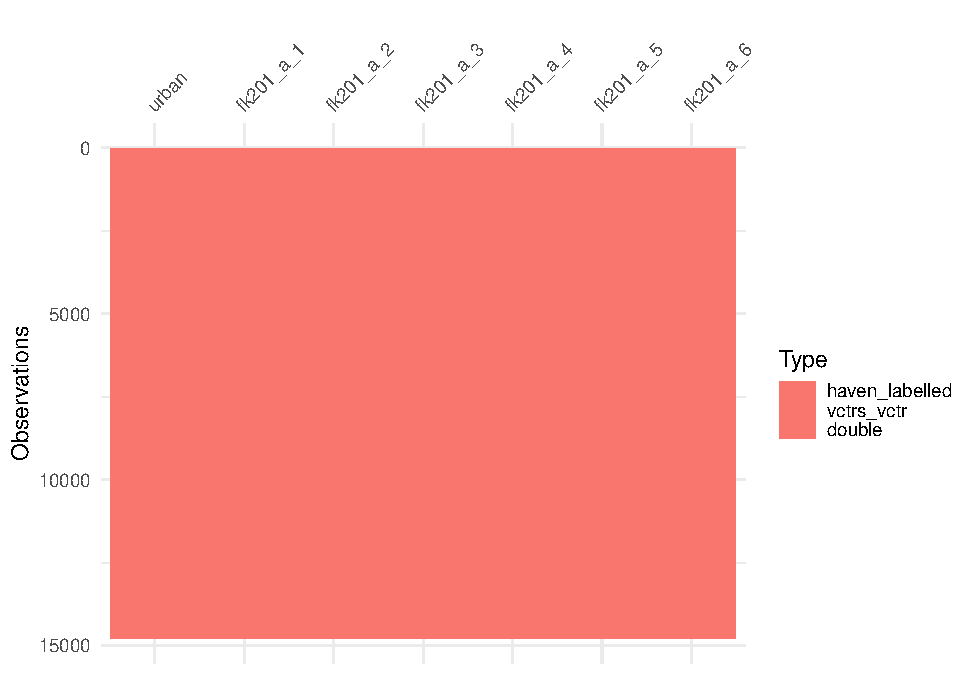
\includegraphics{_main_files/figure-latex/unnamed-chunk-9-1.pdf}

为防止包之间的函数冲突,使用\texttt{conflicted}来prefer到\texttt{dplyr}中的\texttt{filter}。

\begin{Shaded}
\begin{Highlighting}[]
\FunctionTok{library}\NormalTok{(conflicted)}
\FunctionTok{conflict\_prefer}\NormalTok{(}\StringTok{"filter"}\NormalTok{, }\StringTok{"dplyr"}\NormalTok{)}
\end{Highlighting}
\end{Shaded}

\begin{verbatim}
## [conflicted] Will prefer dplyr::filter over any other package.
\end{verbatim}

\begin{Shaded}
\begin{Highlighting}[]
\NormalTok{cfps2010family }\SpecialCharTok{\%\textgreater{}\%}
  \FunctionTok{select}\NormalTok{(urban, }\FunctionTok{starts\_with}\NormalTok{(}\StringTok{"fk2\_s"}\NormalTok{))}\SpecialCharTok{\%\textgreater{}\%}
  \FunctionTok{filter}\NormalTok{(urban }\SpecialCharTok{==} \DecValTok{0}\NormalTok{)}
\end{Highlighting}
\end{Shaded}

\begin{verbatim}
## # A tibble: 7,694 x 6
##    urban     fk2_s_1     fk2_s_2     fk2_s_3     fk2_s_4     fk2_s_5    
##    <dbl+lbl> <dbl+lbl>   <dbl+lbl>   <dbl+lbl>   <dbl+lbl>   <dbl+lbl>  
##  1 0 [乡村]   4 [果园]   -8 [不适用] -8 [不适用] -8 [不适用] -8 [不适用]
##  2 0 [乡村]   2 [旱地]   -8 [不适用] -8 [不适用] -8 [不适用] -8 [不适用]
##  3 0 [乡村]   4 [果园]   -8 [不适用] -8 [不适用] -8 [不适用] -8 [不适用]
##  4 0 [乡村]   4 [果园]   -8 [不适用] -8 [不适用] -8 [不适用] -8 [不适用]
##  5 0 [乡村]  -8 [不适用] -8 [不适用] -8 [不适用] -8 [不适用] -8 [不适用]
##  6 0 [乡村]  -8 [不适用] -8 [不适用] -8 [不适用] -8 [不适用] -8 [不适用]
##  7 0 [乡村]  -8 [不适用] -8 [不适用] -8 [不适用] -8 [不适用] -8 [不适用]
##  8 0 [乡村]   6 [池塘]   -8 [不适用] -8 [不适用] -8 [不适用] -8 [不适用]
##  9 0 [乡村]   4 [果园]   -8 [不适用] -8 [不适用] -8 [不适用] -8 [不适用]
## 10 0 [乡村]  -8 [不适用] -8 [不适用] -8 [不适用] -8 [不适用] -8 [不适用]
## # ... with 7,684 more rows
\end{verbatim}

先找出有经营土地的家户:并不考虑是否是自己拥有还是转租入。

\begin{Shaded}
\begin{Highlighting}[]
\NormalTok{a }\OtherTok{\textless{}{-}}\NormalTok{ cfps2010family }\SpecialCharTok{\%\textgreater{}\%}
  \FunctionTok{select}\NormalTok{(fid,urban, }\FunctionTok{starts\_with}\NormalTok{(}\StringTok{"fk201\_a"}\NormalTok{)) }\SpecialCharTok{\%\textgreater{}\%}
  \FunctionTok{filter\_at}\NormalTok{(}\FunctionTok{vars}\NormalTok{(}\FunctionTok{starts\_with}\NormalTok{(}\StringTok{"fk201\_a"}\NormalTok{)), }\FunctionTok{any\_vars}\NormalTok{(. }\SpecialCharTok{\textgreater{}} \DecValTok{0}\NormalTok{))}
\NormalTok{a}
\end{Highlighting}
\end{Shaded}

\begin{verbatim}
## # A tibble: 7,688 x 8
##    fid       urban     fk201_a_1   fk201_a_2 fk201_~1 fk201_~2 fk201_~3 fk201_~4
##    <dbl+lbl> <dbl+lbl> <dbl+lbl>   <dbl+lbl> <dbl+lb> <dbl+lb> <dbl+lb> <dbl+lb>
##  1 110007    1 [城镇]  -8 [不适用]  2.5    ~ -8 [不~ -8 [不~ -8 [不~ -8 [不~
##  2 120033    1 [城镇]  -8 [不适用] -8 [不适~ -8 [不~  0.900 ~ -8 [不~ -8 [不~
##  3 120073    0 [乡村]  -8 [不适用] -8 [不适~ -8 [不~  5.10  ~ -8 [不~ -8 [不~
##  4 120074    0 [乡村]  -8 [不适用]  1.80   ~ -8 [不~ -8 [不~ -8 [不~ -8 [不~
##  5 120076    0 [乡村]  -8 [不适用] -8 [不适~ -8 [不~  6     ~ -8 [不~ -8 [不~
##  6 120080    0 [乡村]  -8 [不适用] -8 [不适~ -8 [不~ -8 [不~ -8 [不~ 38     ~
##  7 120081    0 [乡村]  -8 [不适用] -8 [不适~ -8 [不~  4     ~ -8 [不~ -8 [不~
##  8 120084    0 [乡村]  -8 [不适用] -8 [不适~ -8 [不~  1.5   ~ -8 [不~ -8 [不~
##  9 120087    0 [乡村]  -8 [不适用] -8 [不适~ -8 [不~  3     ~ -8 [不~ -8 [不~
## 10 120088    0 [乡村]  -8 [不适用]  1.5    ~ -8 [不~ -8 [不~ -8 [不~ -8 [不~
## # ... with 7,678 more rows, and abbreviated variable names 1: fk201_a_3,
## #   2: fk201_a_4, 3: fk201_a_5, 4: fk201_a_6
\end{verbatim}

再将负值转变为0。

\begin{Shaded}
\begin{Highlighting}[]
\NormalTok{a }\SpecialCharTok{\%\textgreater{}\%} \FunctionTok{mutate\_at}\NormalTok{(}\FunctionTok{vars}\NormalTok{(}\FunctionTok{starts\_with}\NormalTok{(}\StringTok{"fk201\_a"}\NormalTok{)), }\FunctionTok{funs}\NormalTok{(}\FunctionTok{replace}\NormalTok{(., . }\SpecialCharTok{\textless{}} \DecValTok{0}\NormalTok{, }\DecValTok{0}\NormalTok{)))}
\end{Highlighting}
\end{Shaded}

\begin{verbatim}
## Warning: `funs()` was deprecated in dplyr 0.8.0.
## i Please use a list of either functions or lambdas:
## 
## # Simple named list: list(mean = mean, median = median)
## 
## # Auto named with `tibble::lst()`: tibble::lst(mean, median)
## 
## # Using lambdas list(~ mean(., trim = .2), ~ median(., na.rm = TRUE))
\end{verbatim}

\begin{verbatim}
## # A tibble: 7,688 x 8
##    fid       urban     fk201_a_1 fk201_a_2 fk201_a_3 fk201_a_4 fk201_a_5 fk201~1
##    <dbl+lbl> <dbl+lbl> <dbl+lbl> <dbl+lbl> <dbl+lbl> <dbl+lbl> <dbl+lbl> <dbl+l>
##  1 110007    1 [城镇]  0         2.5       0         0         0          0     
##  2 120033    1 [城镇]  0         0         0         0.900     0          0     
##  3 120073    0 [乡村]  0         0         0         5.10      0          0     
##  4 120074    0 [乡村]  0         1.80      0         0         0          0     
##  5 120076    0 [乡村]  0         0         0         6         0          0     
##  6 120080    0 [乡村]  0         0         0         0         0         38     
##  7 120081    0 [乡村]  0         0         0         4         0          0     
##  8 120084    0 [乡村]  0         0         0         1.5       0          0     
##  9 120087    0 [乡村]  0         0         0         3         0          0     
## 10 120088    0 [乡村]  0         1.5       0         0         0          0     
## # ... with 7,678 more rows, and abbreviated variable name 1: fk201_a_6
\end{verbatim}

\hypertarget{ux519cux4e1aux751fux4ea7ux6548ux7387}{%
\subsection{农业生产效率}\label{ux519cux4e1aux751fux4ea7ux6548ux7387}}

\begin{Shaded}
\begin{Highlighting}[]
\NormalTok{a }\OtherTok{\textless{}{-}}\NormalTok{ cfps2010family }\SpecialCharTok{\%\textgreater{}\%}
  \FunctionTok{select}\NormalTok{(fid,urban, }\FunctionTok{starts\_with}\NormalTok{(}\StringTok{"fk201\_a"}\NormalTok{),fk3,fk4,fe1)}\SpecialCharTok{\%\textgreater{}\%}
  \FunctionTok{mutate}\NormalTok{(}\AttributeTok{revenue =}\NormalTok{ fk3}\SpecialCharTok{{-}}\NormalTok{fk4)}\SpecialCharTok{\%\textgreater{}\%}
  \FunctionTok{mutate\_at}\NormalTok{(}\FunctionTok{vars}\NormalTok{(}\FunctionTok{starts\_with}\NormalTok{(}\StringTok{"fk201\_a"}\NormalTok{)), }\FunctionTok{funs}\NormalTok{(}\FunctionTok{replace}\NormalTok{(., . }\SpecialCharTok{\textless{}} \DecValTok{0}\NormalTok{, }\DecValTok{0}\NormalTok{)))}\SpecialCharTok{\%\textgreater{}\%}
  \FunctionTok{mutate\_at}\NormalTok{(}\FunctionTok{vars}\NormalTok{(}\StringTok{"revenue"}\NormalTok{), }\FunctionTok{funs}\NormalTok{(}\FunctionTok{replace}\NormalTok{(., . }\SpecialCharTok{\textless{}} \DecValTok{0}\NormalTok{, }\DecValTok{0}\NormalTok{)))}\SpecialCharTok{\%\textgreater{}\%}
\NormalTok{  dplyr}\SpecialCharTok{::}\FunctionTok{filter}\NormalTok{(revenue}\SpecialCharTok{\textgreater{}}\DecValTok{0}\NormalTok{)}
\end{Highlighting}
\end{Shaded}

\begin{verbatim}
## Warning: `funs()` was deprecated in dplyr 0.8.0.
## i Please use a list of either functions or lambdas:
## 
## # Simple named list: list(mean = mean, median = median)
## 
## # Auto named with `tibble::lst()`: tibble::lst(mean, median)
## 
## # Using lambdas list(~ mean(., trim = .2), ~ median(., na.rm = TRUE))
\end{verbatim}

\begin{verbatim}
## Warning: `funs()` was deprecated in dplyr 0.8.0.
## i Please use a list of either functions or lambdas:
## 
## # Simple named list: list(mean = mean, median = median)
## 
## # Auto named with `tibble::lst()`: tibble::lst(mean, median)
## 
## # Using lambdas list(~ mean(., trim = .2), ~ median(., na.rm = TRUE))
\end{verbatim}

\begin{Shaded}
\begin{Highlighting}[]
\NormalTok{a}
\end{Highlighting}
\end{Shaded}

\begin{verbatim}
## # A tibble: 6,093 x 12
##    fid       urban   fk201~1 fk201~2 fk201~3 fk201~4 fk201~5 fk201~6 fk3   fk4  
##    <dbl+lbl> <dbl+l> <dbl+l> <dbl+l> <dbl+l> <dbl+l> <dbl+l> <dbl+l> <dbl> <dbl>
##  1 110007    1 [城~ 0       2.5     0       0       0       0        1800   500
##  2 120033    1 [城~ 0       0       0       0.900   0       0       16000  1500
##  3 120074    0 [乡~ 0       1.80    0       0       0       0        2100   900
##  4 120075    0 [乡~ 0       0       0       0       0       0       15000  5500
##  5 120076    0 [乡~ 0       0       0       6       0       0       30000 12000
##  6 120081    0 [乡~ 0       0       0       4       0       0       32000  6000
##  7 120084    0 [乡~ 0       0       0       1.5     0       0        7000  4000
##  8 120087    0 [乡~ 0       0       0       3       0       0       25000  5000
##  9 120088    0 [乡~ 0       1.5     0       0       0       0        5300   300
## 10 120090    0 [乡~ 0       0       0       4.5     0       0       26000  6000
## # ... with 6,083 more rows, 2 more variables: fe1 <dbl+lbl>, revenue <dbl>, and
## #   abbreviated variable names 1: fk201_a_1, 2: fk201_a_2, 3: fk201_a_3,
## #   4: fk201_a_4, 5: fk201_a_5, 6: fk201_a_6
\end{verbatim}

一个有效的建议是在对原始数据进行操作时候,尽量保证原始数据的不变,再通过\texttt{\%\textgreater{}\%}进行传导到新的数据框中。

我们计算农业生产效率的方法有很多这里主要参考的是一些主流的做法:将单位面积纯利润作为效率的衡量指标

\begin{Shaded}
\begin{Highlighting}[]
\NormalTok{a}\SpecialCharTok{\%\textgreater{}\%}
  \FunctionTok{mutate}\NormalTok{(}\AttributeTok{landsum =} \FunctionTok{rowSums}\NormalTok{(.[}\DecValTok{2}\SpecialCharTok{:}\DecValTok{7}\NormalTok{]))}\SpecialCharTok{\%\textgreater{}\%}
  \FunctionTok{filter}\NormalTok{(landsum}\SpecialCharTok{\textgreater{}}\DecValTok{0}\NormalTok{)}\SpecialCharTok{\%\textgreater{}\%}
  \FunctionTok{mutate}\NormalTok{(}\AttributeTok{rates =}\NormalTok{ revenue}\SpecialCharTok{/}\NormalTok{landsum)}\OtherTok{{-}\textgreater{}}\NormalTok{a1}
\NormalTok{a1}
\end{Highlighting}
\end{Shaded}

\begin{verbatim}
## # A tibble: 6,048 x 14
##    fid       urban   fk201~1 fk201~2 fk201~3 fk201~4 fk201~5 fk201~6 fk3   fk4  
##    <dbl+lbl> <dbl+l> <dbl+l> <dbl+l> <dbl+l> <dbl+l> <dbl+l> <dbl+l> <dbl> <dbl>
##  1 110007    1 [城~ 0       2.5     0       0       0       0        1800   500
##  2 120033    1 [城~ 0       0       0       0.900   0       0       16000  1500
##  3 120074    0 [乡~ 0       1.80    0       0       0       0        2100   900
##  4 120076    0 [乡~ 0       0       0       6       0       0       30000 12000
##  5 120081    0 [乡~ 0       0       0       4       0       0       32000  6000
##  6 120084    0 [乡~ 0       0       0       1.5     0       0        7000  4000
##  7 120087    0 [乡~ 0       0       0       3       0       0       25000  5000
##  8 120088    0 [乡~ 0       1.5     0       0       0       0        5300   300
##  9 120090    0 [乡~ 0       0       0       4.5     0       0       26000  6000
## 10 120091    0 [乡~ 0       0       0       4       0       0       30000  5000
## # ... with 6,038 more rows, 4 more variables: fe1 <dbl+lbl>, revenue <dbl>,
## #   landsum <dbl>, rates <dbl>, and abbreviated variable names 1: fk201_a_1,
## #   2: fk201_a_2, 3: fk201_a_3, 4: fk201_a_4, 5: fk201_a_5, 6: fk201_a_6
\end{verbatim}

\hypertarget{ux6d41ux52a8ux4ebaux53e3}{%
\subsection{流动人口}\label{ux6d41ux52a8ux4ebaux53e3}}

我们可以用外出打工在家庭人口中的占比来测算流动率。


\includegraphics{image/fe1.png}

\begin{Shaded}
\begin{Highlighting}[]
\FunctionTok{library}\NormalTok{(conflicted)}
\FunctionTok{conflict\_prefer}\NormalTok{(}\StringTok{\textquotesingle{}filter\textquotesingle{}}\NormalTok{,}\StringTok{"dplyr"}\NormalTok{)}
\end{Highlighting}
\end{Shaded}

\begin{verbatim}
## [conflicted] Removing existing preference.
## [conflicted] Will prefer dplyr::filter over any other package.
\end{verbatim}

\begin{Shaded}
\begin{Highlighting}[]
\NormalTok{a1}\SpecialCharTok{\%\textgreater{}\%}
  \FunctionTok{filter}\NormalTok{(fe1}\SpecialCharTok{!=}\DecValTok{5}\NormalTok{)}\OtherTok{{-}\textgreater{}}\NormalTok{a2}
\NormalTok{a2}\SpecialCharTok{$}\NormalTok{fe1[a2}\SpecialCharTok{$}\NormalTok{fe1}\SpecialCharTok{==}\DecValTok{3}\NormalTok{] }\OtherTok{\textless{}{-}} \DecValTok{0}
\NormalTok{a2}\SpecialCharTok{\%\textgreater{}\%}
  \FunctionTok{select}\NormalTok{(rates,fe1)}
\end{Highlighting}
\end{Shaded}

\begin{verbatim}
## # A tibble: 6,017 x 2
##    rates fe1      
##    <dbl> <dbl+lbl>
##  1  371. 0        
##  2 7632. 0        
##  3  667. 0        
##  4 3000  1 [有]   
##  5 6500  0        
##  6 2000  0        
##  7 6667. 0        
##  8 3333. 0        
##  9 4444. 0        
## 10 6250  0        
## # ... with 6,007 more rows
\end{verbatim}

\hypertarget{ux6a21ux578bux5efaux7acb}{%
\section{模型建立}\label{ux6a21ux578bux5efaux7acb}}

我们试图考察关于流动人口与农业生产效率之间的关系:

\begin{Shaded}
\begin{Highlighting}[]
\NormalTok{reg }\OtherTok{\textless{}{-}} \FunctionTok{lm}\NormalTok{(}\AttributeTok{data =}\NormalTok{ a2,fe1}\SpecialCharTok{\textasciitilde{}}\NormalTok{rates)}
\FunctionTok{summary}\NormalTok{(reg)}
\end{Highlighting}
\end{Shaded}

\begin{verbatim}
## 
## Call:
## lm(formula = fe1 ~ rates, data = a2)
## 
## Residuals:
##     Min      1Q  Median      3Q     Max 
## -0.3873 -0.3869 -0.3862  0.6130  0.9042 
## 
## Coefficients:
##               Estimate Std. Error t value Pr(>|t|)    
## (Intercept)  3.873e-01  6.329e-03    61.2   <2e-16 ***
## rates       -8.330e-07  6.409e-07    -1.3    0.194    
## ---
## Signif. codes:  0 '***' 0.001 '**' 0.01 '*' 0.05 '.' 0.1 ' ' 1
## 
## Residual standard error: 0.4869 on 6015 degrees of freedom
## Multiple R-squared:  0.0002807,  Adjusted R-squared:  0.0001145 
## F-statistic: 1.689 on 1 and 6015 DF,  p-value: 0.1938
\end{verbatim}

不过不显著。。。不过系数上看是一个较为合理的存在(效率上升,抑制外出)。对于一个想要看星星的reg monkey来说极其苦恼。我们可以考虑换一个变量:一篇2016年在《中国农村经济》的文章研究``非农就业、土地流转与农业生产效率变化''利用的是非农就业来考察劳动生产率(同样也是用单位土地的农产品收入来测算)就较为显著,主要的差别在于非农就业数量来测度,并非一个虚拟变量。
还有一个可能是在先前的数据处理中存在一定的问题,比如是否将未从事农业活动的家户过滤进来。

\begin{Shaded}
\begin{Highlighting}[]
\NormalTok{cfps2010family}\SpecialCharTok{\%\textgreater{}\%}
  \FunctionTok{select}\NormalTok{(fid,familysize,}\FunctionTok{starts\_with}\NormalTok{(}\StringTok{"fu1\_s"}\NormalTok{))}\SpecialCharTok{\%\textgreater{}\%}
  \FunctionTok{mutate\_at}\NormalTok{(}\FunctionTok{vars}\NormalTok{(}\FunctionTok{starts\_with}\NormalTok{(}\StringTok{"fu1\_s"}\NormalTok{)), }\FunctionTok{funs}\NormalTok{(}\FunctionTok{replace}\NormalTok{(., . }\SpecialCharTok{\textless{}} \DecValTok{0}\NormalTok{, }\DecValTok{0}\NormalTok{)))}\SpecialCharTok{\%\textgreater{}\%}
  \FunctionTok{mutate\_at}\NormalTok{(}\FunctionTok{vars}\NormalTok{(}\FunctionTok{starts\_with}\NormalTok{(}\StringTok{"fu1\_s"}\NormalTok{)), }\FunctionTok{funs}\NormalTok{(}\FunctionTok{replace}\NormalTok{(., . }\SpecialCharTok{\textgreater{}=}\DecValTok{1}\NormalTok{, }\DecValTok{1}\NormalTok{)))}\OtherTok{{-}\textgreater{}}\NormalTok{b1}
\end{Highlighting}
\end{Shaded}

\begin{verbatim}
## Warning: `funs()` was deprecated in dplyr 0.8.0.
## i Please use a list of either functions or lambdas:
## 
## # Simple named list: list(mean = mean, median = median)
## 
## # Auto named with `tibble::lst()`: tibble::lst(mean, median)
## 
## # Using lambdas list(~ mean(., trim = .2), ~ median(., na.rm = TRUE))
\end{verbatim}

\begin{verbatim}
## Warning: `funs()` was deprecated in dplyr 0.8.0.
## i Please use a list of either functions or lambdas:
## 
## # Simple named list: list(mean = mean, median = median)
## 
## # Auto named with `tibble::lst()`: tibble::lst(mean, median)
## 
## # Using lambdas list(~ mean(., trim = .2), ~ median(., na.rm = TRUE))
\end{verbatim}

并不建议一次性将所有变换都做完,之后再检查是非常痛苦的。。。

\begin{Shaded}
\begin{Highlighting}[]
\NormalTok{b1}\SpecialCharTok{\%\textgreater{}\%}
  \FunctionTok{mutate}\NormalTok{(}\AttributeTok{mig =} \FunctionTok{rowSums}\NormalTok{(.[}\DecValTok{3}\SpecialCharTok{:}\DecValTok{14}\NormalTok{]))}\SpecialCharTok{\%\textgreater{}\%}
  \FunctionTok{select}\NormalTok{(fid,familysize,mig)}\SpecialCharTok{\%\textgreater{}\%}
  \FunctionTok{mutate}\NormalTok{(}\AttributeTok{mig\_rate =}\NormalTok{ mig}\SpecialCharTok{/}\NormalTok{familysize)}\SpecialCharTok{\%\textgreater{}\%}
  \FunctionTok{filter}\NormalTok{(mig\_rate}\SpecialCharTok{\textless{}=}\DecValTok{1}\SpecialCharTok{\&}\NormalTok{mig\_rate}\SpecialCharTok{\textgreater{}=}\DecValTok{0}\NormalTok{)}\OtherTok{{-}\textgreater{}}\NormalTok{b2}\CommentTok{\# 剔除异常值}
\FunctionTok{barplot}\NormalTok{(}\FunctionTok{table}\NormalTok{(b2}\SpecialCharTok{$}\NormalTok{mig\_rate))}
\end{Highlighting}
\end{Shaded}

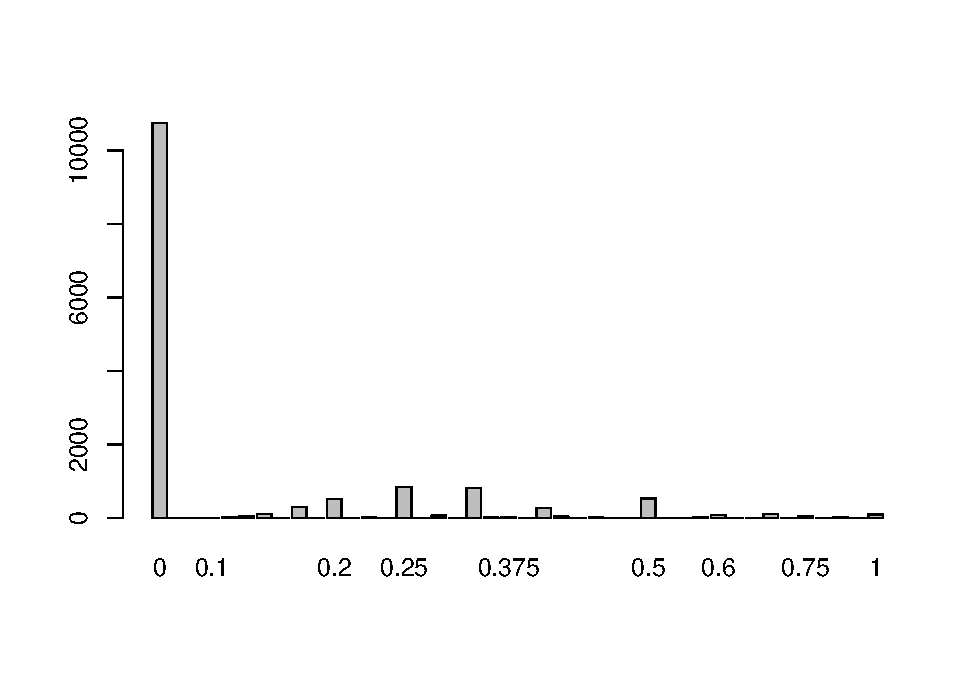
\includegraphics{_main_files/figure-latex/unnamed-chunk-18-1.pdf}

\begin{Shaded}
\begin{Highlighting}[]
\FunctionTok{dim}\NormalTok{(b2)}
\end{Highlighting}
\end{Shaded}

\begin{verbatim}
## [1] 14795     4
\end{verbatim}

\begin{Shaded}
\begin{Highlighting}[]
\NormalTok{b3 }\OtherTok{\textless{}{-}} \FunctionTok{merge}\NormalTok{(a2,b2,}\AttributeTok{by=}\StringTok{"fid"}\NormalTok{)}
\NormalTok{reg2 }\OtherTok{\textless{}{-}} \FunctionTok{lm}\NormalTok{(}\AttributeTok{data =}\NormalTok{ b3,mig\_rate}\SpecialCharTok{\textasciitilde{}}\NormalTok{rates)}
\FunctionTok{summary}\NormalTok{(reg2)}
\end{Highlighting}
\end{Shaded}

\begin{verbatim}
## 
## Call:
## lm(formula = mig_rate ~ rates, data = b3)
## 
## Residuals:
##     Min      1Q  Median      3Q     Max 
## -0.1249 -0.1248 -0.1247  0.1251  0.8760 
## 
## Coefficients:
##               Estimate Std. Error t value Pr(>|t|)    
## (Intercept)  1.249e-01  2.384e-03   52.40   <2e-16 ***
## rates       -2.029e-07  2.415e-07   -0.84    0.401    
## ---
## Signif. codes:  0 '***' 0.001 '**' 0.01 '*' 0.05 '.' 0.1 ' ' 1
## 
## Residual standard error: 0.1834 on 6015 degrees of freedom
## Multiple R-squared:  0.0001174,  Adjusted R-squared:  -4.887e-05 
## F-statistic: 0.706 on 1 and 6015 DF,  p-value: 0.4008
\end{verbatim}

p值比之前还更大了。。。上述提到的文章的核心解释变量是非农占家庭劳动力比例,但目前还不知咋构建的。。。想到了再补上去。

\hypertarget{ux6587ux732eux590dux523bux52b3ux52a8ux529bux6d41ux52a8ux5982ux4f55ux5f71ux54cdux519cux6237ux501fux8d37}{%
\chapter{文献复刻:《劳动力流动如何影响农户借贷》}\label{ux6587ux732eux590dux523bux52b3ux52a8ux529bux6d41ux52a8ux5982ux4f55ux5f71ux54cdux519cux6237ux501fux8d37}}

\hypertarget{ux6587ux732eux56deux987e}{%
\section{文献回顾}\label{ux6587ux732eux56deux987e}}

\href{https://www.cnki.com.cn/Article/CJFDTOTAL-SJJJ202112006.htm}{这篇文章}主要发现劳动力流动导致农户借出的概率和金额显著增加。

\begin{itemize}
\item
  核心的被解释变量为家庭是否有借给亲戚、朋友等的借出款项和为家庭人均借出金额的对数值。降低极端值影响,进行上下2\%缩尾处理。
\item
  劳动力流动:是否有劳动力流动以及家庭劳动力流动人数。
\item
  控制变量:
\end{itemize}

\hypertarget{ux6570ux636eux5904ux7406}{%
\section{数据处理}\label{ux6570ux636eux5904ux7406}}

加载cfps2018数据:

\hypertarget{ux7edfux8ba1ux63cfux8ff0}{%
\section{统计描述}\label{ux7edfux8ba1ux63cfux8ff0}}

\hypertarget{ux6a21ux578bux8bbeux5b9a}{%
\section{模型设定}\label{ux6a21ux578bux8bbeux5b9a}}

\hypertarget{culture}{%
\chapter{宗族文化}\label{culture}}

对于宗族文化的研究近些年一直是较为火热的研究热点\citep{Cao2022},\citep{Hanetsu2019a},\citep{ZhangShinYi2021a},\citep{ZhangKawagawa2017},\citep{ZHANG2020100}和\citep{FAN2023457}。但对于宗族文化的测度方法又各具差异,比如 \citet{ZHANG2020100}, \citet{Cao2022} 和 \citet{FAN2023457} 都是使用上海古籍出版社的县地方族谱数据来测量宗族文化,\citet{ZhangKawagawa2017} 使用的是CFPS的数据来测量;\citet{ZhangShinYi2021a} 使用的是地方的前三姓氏来作为度量,数据来源是2005年的1\%人口抽样调查数据。数据质量上,直观感受是上海古籍出版社的数据会优于其他几个。

\hypertarget{ux6570ux636eux8f7dux5165}{%
\section{数据载入}\label{ux6570ux636eux8f7dux5165}}

如何在R中没有任何资源的前提下进行关于宗族文化的测度,我先试了做法最为简便的,城市的前三姓氏我翻遍了所有变量都没找到姓氏的变量;后面又看了下上海古籍出版社数据,数据量太大,估计需要爬虫等黑科技,遂又放弃,之后只有选择CFPS,之后也并不很顺利。

\begin{Shaded}
\begin{Highlighting}[]
\FunctionTok{library}\NormalTok{(haven)}
\end{Highlighting}
\end{Shaded}

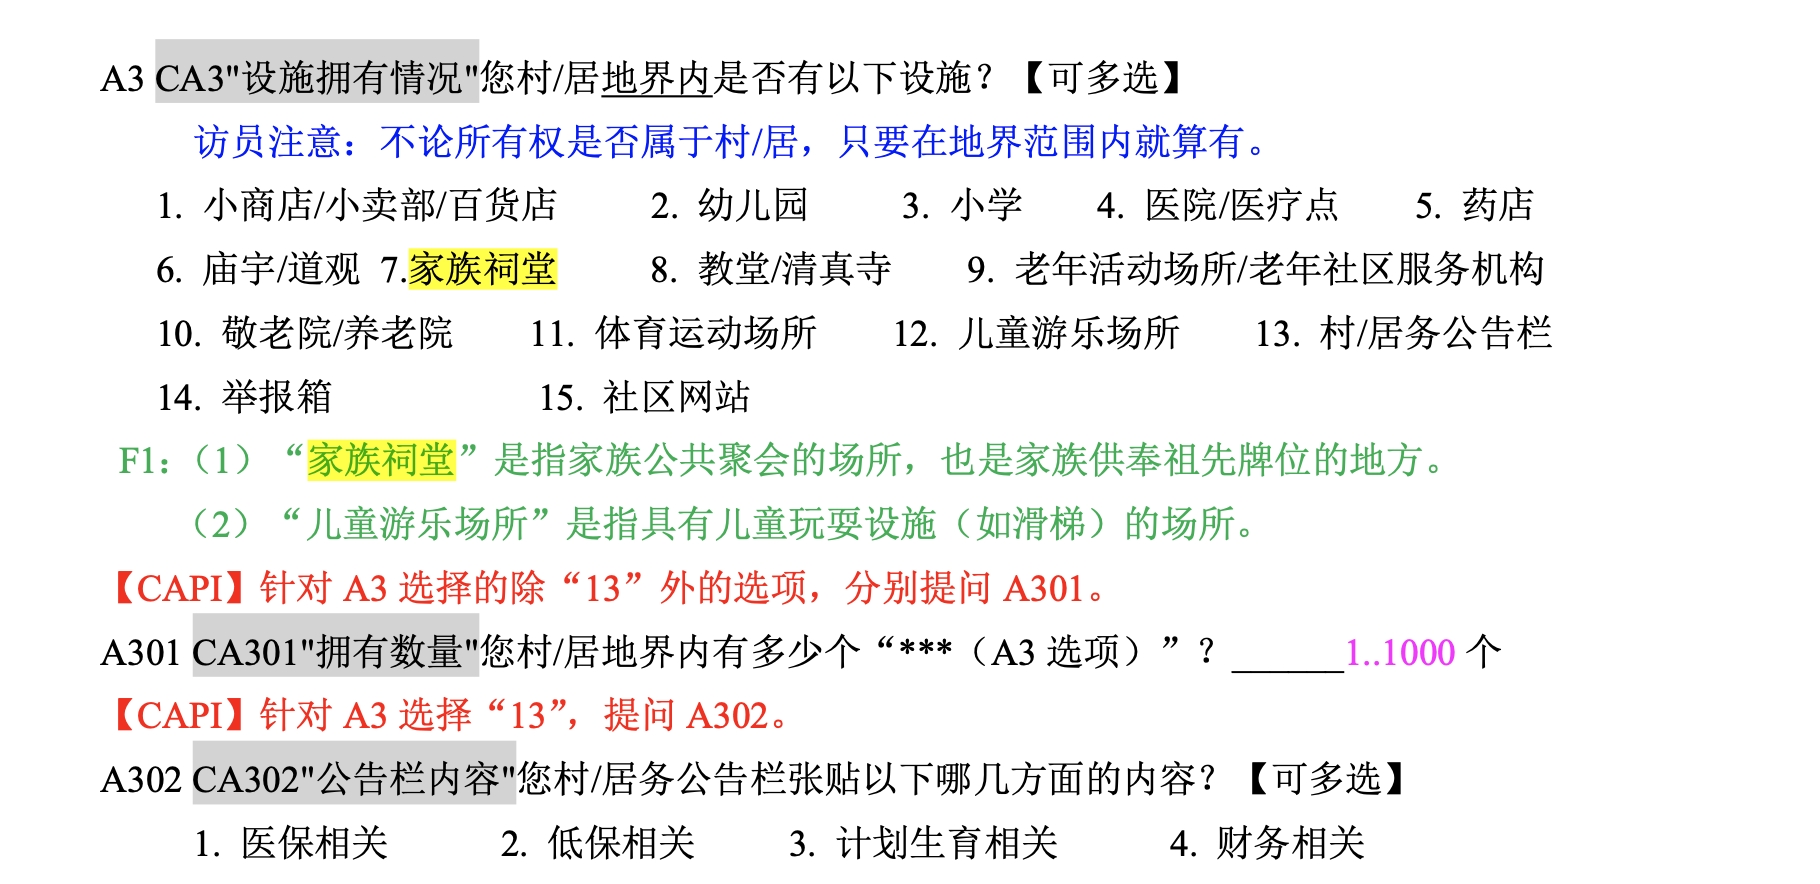
\includegraphics{image/q1.png}

\begin{Shaded}
\begin{Highlighting}[]
\NormalTok{cfps2010comm }\OtherTok{\textless{}{-}} \FunctionTok{read\_dta}\NormalTok{(}\StringTok{"/Users/a182501/rproject/cfps/data/社区数据cfps/cfps2010comm\_201906.dta"}\NormalTok{)}
\NormalTok{cfps2010comm}\SpecialCharTok{\%\textgreater{}\%}
  \FunctionTok{select}\NormalTok{(cid,provcd,countyid,cyear,cmonth,ca3\_s\_6,ca3\_s\_7)}\OtherTok{{-}\textgreater{}}\NormalTok{df1}
\FunctionTok{head}\NormalTok{(df1)}
\end{Highlighting}
\end{Shaded}

\begin{verbatim}
## # A tibble: 6 x 7
##   cid       provcd        countyid  cyear     cmonth ca3_s_6            ca3_s_7 
##   <dbl+lbl> <dbl+lbl>     <dbl+lbl> <dbl+lbl>  <dbl> <dbl+lbl>          <dbl+lb>
## 1 13200     12 [天津市]    79       2010          10 -8 [不适用]      ~ -8 [不~
## 2 13190     12 [天津市]    79       2010          10  9 [老年活动场所/~ 13 [村/~
## 3 12780     14 [山西省]    69       2010          10  8 [教堂/清真寺] ~ 10 [敬~
## 4 21340     44 [广东省]   116       2010          10  9 [老年活动场所/~ 13 [村/~
## 5 12260     23 [黑龙江省]  56       2010           9 -8 [不适用]      ~ -8 [不~
## 6 21640     44 [广东省]   123       2010          10  7 [家族祠堂]    ~ 11 [体~
\end{verbatim}

\begin{Shaded}
\begin{Highlighting}[]
\FunctionTok{dim}\NormalTok{(df1)}
\end{Highlighting}
\end{Shaded}

\begin{verbatim}
## [1] 635   7
\end{verbatim}

\begin{Shaded}
\begin{Highlighting}[]
\NormalTok{cfps2010comm}\SpecialCharTok{$}\NormalTok{ca3\_s\_6[}\FunctionTok{which}\NormalTok{(df1}\SpecialCharTok{$}\NormalTok{ca3\_s\_6}\SpecialCharTok{=={-}}\DecValTok{8}\NormalTok{)]}\OtherTok{=}\DecValTok{0}
\NormalTok{cfps2010comm}\SpecialCharTok{$}\NormalTok{ca3\_s\_7[}\FunctionTok{which}\NormalTok{(df1}\SpecialCharTok{$}\NormalTok{ca3\_s\_7}\SpecialCharTok{=={-}}\DecValTok{8}\NormalTok{)]}\OtherTok{=}\DecValTok{0}
\FunctionTok{table}\NormalTok{(cfps2010comm}\SpecialCharTok{$}\NormalTok{ca3\_s\_7)}
\end{Highlighting}
\end{Shaded}

\begin{verbatim}
## 
##   0   2   7   8   9  10  11  12  13  14  15 
## 262   2  14   6  41  26  66  26 106  68  18
\end{verbatim}

\begin{Shaded}
\begin{Highlighting}[]
\FunctionTok{table}\NormalTok{(cfps2010comm}\SpecialCharTok{$}\NormalTok{ca3\_s\_6)}
\end{Highlighting}
\end{Shaded}

\begin{verbatim}
## 
##   0   2   3   5   6   7   8   9  10  11  12  13  14  15 
## 172   1   1   1  47  23  23  92  24  58  21  94  72   6
\end{verbatim}

\begin{Shaded}
\begin{Highlighting}[]
\FunctionTok{na.omit}\NormalTok{(df1)}
\end{Highlighting}
\end{Shaded}

\begin{verbatim}
## # A tibble: 635 x 7
##    cid       provcd        countyid  cyear     cmonth ca3_s_6           ca3_s_7 
##    <dbl+lbl> <dbl+lbl>     <dbl+lbl> <dbl+lbl>  <dbl> <dbl+lbl>         <dbl+lb>
##  1 13200     12 [天津市]    79       2010          10 -8 [不适用]     ~ -8 [不~
##  2 13190     12 [天津市]    79       2010          10  9 [老年活动场所~ 13 [村/~
##  3 12780     14 [山西省]    69       2010          10  8 [教堂/清真寺]~ 10 [敬~
##  4 21340     44 [广东省]   116       2010          10  9 [老年活动场所~ 13 [村/~
##  5 12260     23 [黑龙江省]  56       2010           9 -8 [不适用]     ~ -8 [不~
##  6 21640     44 [广东省]   123       2010          10  7 [家族祠堂]   ~ 11 [体~
##  7 21730     44 [广东省]   126       2010          10 -8 [不适用]     ~ -8 [不~
##  8 22523     62 [甘肃省]   145       2010           9 -8 [不适用]     ~ -8 [不~
##  9 10930     52 [贵州省]    24       2010          10 12 [儿童游乐场所~ 13 [村/~
## 10 10100     34 [安徽省]     3       2010          10  6 [庙宇/道观]  ~ 10 [敬~
## # ... with 625 more rows
\end{verbatim}

\begin{Shaded}
\begin{Highlighting}[]
\FunctionTok{dim}\NormalTok{(df1)}
\end{Highlighting}
\end{Shaded}

\begin{verbatim}
## [1] 635   7
\end{verbatim}

根据社区问卷手册,我们可以指导

\begin{Shaded}
\begin{Highlighting}[]
\FunctionTok{library}\NormalTok{(dplyr)}
\NormalTok{cfps2010comm}\SpecialCharTok{\%\textgreater{}\%}
  \FunctionTok{group\_by}\NormalTok{(provcd)}\SpecialCharTok{\%\textgreater{}\%}
\NormalTok{  dplyr}\SpecialCharTok{::}\FunctionTok{summarise}\NormalTok{(}\AttributeTok{x1=}\FunctionTok{sum}\NormalTok{(ca3\_s\_6),}\AttributeTok{x2=}\FunctionTok{sum}\NormalTok{(ca3\_s\_7))}\OtherTok{{-}\textgreater{}}\NormalTok{df2}
\NormalTok{df2}
\end{Highlighting}
\end{Shaded}

\begin{verbatim}
## # A tibble: 25 x 3
##    provcd           x1    x2
##    <dbl+lbl>     <dbl> <dbl>
##  1 11 [北京市]      27    14
##  2 12 [天津市]       9    13
##  3 13 [河北省]     216   178
##  4 14 [山西省]     207   220
##  5 21 [辽宁省]     525   511
##  6 22 [吉林省]      97   112
##  7 23 [黑龙江省]   159   155
##  8 31 [上海市]     495   386
##  9 32 [江苏省]     127   117
## 10 33 [浙江省]     111   126
## # ... with 15 more rows
\end{verbatim}

\hypertarget{ux53efux89c6ux5316}{%
\section{可视化}\label{ux53efux89c6ux5316}}

\begin{Shaded}
\begin{Highlighting}[]
\FunctionTok{library}\NormalTok{(ggplot2)}
\FunctionTok{ggplot}\NormalTok{(df2)}\SpecialCharTok{+}
  \FunctionTok{geom\_point}\NormalTok{(}\FunctionTok{aes}\NormalTok{(}\AttributeTok{x=}\NormalTok{x1,}\AttributeTok{y=}\NormalTok{x2))}\SpecialCharTok{+}
  \FunctionTok{geom\_smooth}\NormalTok{(}\AttributeTok{method =} \StringTok{\textquotesingle{}lm\textquotesingle{}}\NormalTok{,}\FunctionTok{aes}\NormalTok{(}\AttributeTok{x=}\NormalTok{x1,}\AttributeTok{y=}\NormalTok{x2))}
\end{Highlighting}
\end{Shaded}

\begin{verbatim}
## `geom_smooth()` using formula = 'y ~ x'
\end{verbatim}

\begin{figure}

{\centering 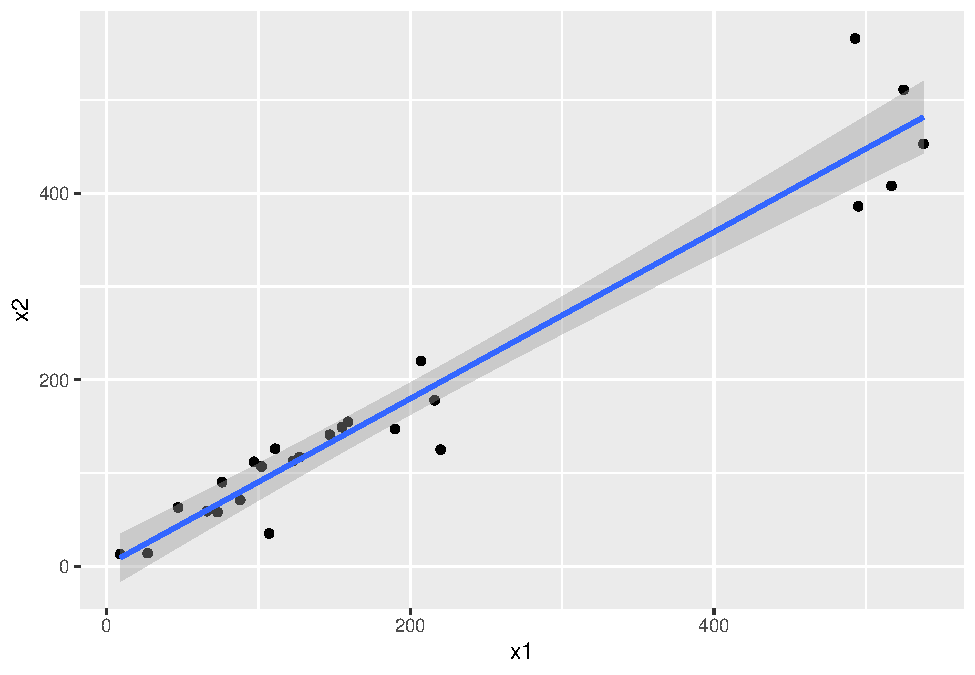
\includegraphics{_main_files/figure-latex/as-1} 

}

\caption{祠堂与族谱}\label{fig:as}
\end{figure}

\hypertarget{ux5730ux56fe}{%
\section{地图}\label{ux5730ux56fe}}

将论文图表绘制在图上。

\begin{Shaded}
\begin{Highlighting}[]
\NormalTok{d }\OtherTok{\textless{}{-}} \FunctionTok{attributes}\NormalTok{(df2}\SpecialCharTok{$}\NormalTok{provcd)}\SpecialCharTok{$}\NormalTok{labels}
\NormalTok{d }\OtherTok{\textless{}{-}} \FunctionTok{as.data.frame}\NormalTok{(d)}
\NormalTok{d2 }\OtherTok{\textless{}{-}} \FunctionTok{rownames}\NormalTok{(d)}
\NormalTok{d3 }\OtherTok{\textless{}{-}} \FunctionTok{cbind}\NormalTok{(d,d2)}
\FunctionTok{colnames}\NormalTok{(d3) }\OtherTok{\textless{}{-}} \FunctionTok{c}\NormalTok{(}\StringTok{"provcd"}\NormalTok{,}\StringTok{"label"}\NormalTok{)}
\NormalTok{d4 }\OtherTok{\textless{}{-}} \FunctionTok{merge}\NormalTok{(df2,d3,}\AttributeTok{by =} \StringTok{"provcd"}\NormalTok{)}
\NormalTok{d4}
\end{Highlighting}
\end{Shaded}

\begin{verbatim}
##    provcd  x1  x2          label
## 1      11  27  14         北京市
## 2      12   9  13         天津市
## 3      13 216 178         河北省
## 4      14 207 220         山西省
## 5      21 525 511         辽宁省
## 6      22  97 112         吉林省
## 7      23 159 155       黑龙江省
## 8      31 495 386         上海市
## 9      32 127 117         江苏省
## 10     33 111 126         浙江省
## 11     34 123 113         安徽省
## 12     35  47  63         福建省
## 13     36 102 107         江西省
## 14     37 220 125         山东省
## 15     41 538 453         河南省
## 16     42  76  90         湖北省
## 17     43 190 147         湖南省
## 18     44 493 566         广东省
## 19     45 107  35 广西壮族自治区
## 20     50  66  59         重庆市
## 21     51 155 149         四川省
## 22     52  88  71         贵州省
## 23     53 147 141         云南省
## 24     61  73  58         陕西省
## 25     62 517 408         甘肃省
\end{verbatim}

json数据来源于\href{http://datav.aliyun.com/portal/school/atlas/area_selector}{阿里 DataV 数据可视化平台},能够在多个行政层级绘制中国地图。

\begin{Shaded}
\begin{Highlighting}[]
\FunctionTok{library}\NormalTok{(echarts4r.maps)}
\FunctionTok{library}\NormalTok{(echarts4r)}
\FunctionTok{colnames}\NormalTok{(d4) }\OtherTok{\textless{}{-}} \FunctionTok{c}\NormalTok{(}\StringTok{"provcd"}\NormalTok{,}\StringTok{"value1"}\NormalTok{,}\StringTok{"value2"}\NormalTok{,}\StringTok{"region"}\NormalTok{)}
\NormalTok{china\_map }\OtherTok{\textless{}{-}}\NormalTok{ jsonlite}\SpecialCharTok{::}\FunctionTok{read\_json}\NormalTok{(}\StringTok{"rep.json"}\NormalTok{)}
\NormalTok{d4 }\SpecialCharTok{\%\textgreater{}\%}
  \FunctionTok{e\_charts}\NormalTok{(region)}\SpecialCharTok{\%\textgreater{}\%}
  \FunctionTok{e\_map\_register}\NormalTok{(}\StringTok{"China2"}\NormalTok{, china\_map) }\SpecialCharTok{\%\textgreater{}\%}
  \FunctionTok{e\_map}\NormalTok{(value1, }\AttributeTok{map =} \StringTok{"China2"}\NormalTok{) }\SpecialCharTok{\%\textgreater{}\%}
  \FunctionTok{e\_visual\_map}\NormalTok{(value1)}
\end{Highlighting}
\end{Shaded}


\includegraphics{_main_files/figure-latex/unnamed-chunk-26-1.pdf}

\begin{Shaded}
\begin{Highlighting}[]
\NormalTok{d4 }\SpecialCharTok{\%\textgreater{}\%}
  \FunctionTok{e\_charts}\NormalTok{(region)}\SpecialCharTok{\%\textgreater{}\%}
  \FunctionTok{e\_map\_register}\NormalTok{(}\StringTok{"China2"}\NormalTok{, china\_map) }\SpecialCharTok{\%\textgreater{}\%}
  \FunctionTok{e\_map}\NormalTok{(value2, }\AttributeTok{map =} \StringTok{"China2"}\NormalTok{) }\SpecialCharTok{\%\textgreater{}\%}
  \FunctionTok{e\_visual\_map}\NormalTok{(value2)}
\end{Highlighting}
\end{Shaded}


\includegraphics{_main_files/figure-latex/unnamed-chunk-27-1.pdf}

上面的数据还是挺让人吃惊的,一般会认为宗族文化会在南方更为发达,包括修建祠堂上,我们通过图 \ref{fig:as} 中知道祠堂与家谱是基本上在省层面是正相关的,但地域上呈现了较大的差异。可能是与抽样方法有关,需要进一步的处理。

\hypertarget{ux5176ux4ed6ux6570ux636eux6e90}{%
\section{其他数据源}\label{ux5176ux4ed6ux6570ux636eux6e90}}

目前学界用的较为广泛的是通过上海家族族谱来测算宗族文化,也就是看一个地方的族谱的密度来作为宗族文化的代理变量,代表性学者有浙大的\href{https://scholar.google.com/citations?user=_YWE1C4AAAAJ\&hl=en\&oi=ao}{张川川老师},他目前发表的关于宗族文化的论文有\citep{Cao2022}, \citep{ZHANG2020100}, \citep{ZhangKawagawa2017}。
很巧,他和合作者\href{https://yiqingxu.org/}{Yiqin Xu}和博士生曹家瑞在JDE刊发的论文有\href{https://yiqingxu.org/papers/english/2022_famine/replication.zip}{replicate file}(可直接下载)

但图中的图是使用ArcGIS来实现的,这里试图通过R来进行复刻。

\hypertarget{charls}{%
\chapter{CHARLS}\label{charls}}

\href{http://charls.pku.edu.cn/}{CHARLS}是中国中老年人调查数据,由北大发起的关于中国中老年人的社会调查。

\hypertarget{ux6570ux636eux5bfcux5165}{%
\section{数据导入}\label{ux6570ux636eux5bfcux5165}}

\begin{Shaded}
\begin{Highlighting}[]
\FunctionTok{library}\NormalTok{(haven)}
\end{Highlighting}
\end{Shaded}

\begin{Shaded}
\begin{Highlighting}[]
\FunctionTok{getwd}\NormalTok{()}
\end{Highlighting}
\end{Shaded}

\begin{verbatim}
## [1] "/Users/a182501/rproject/cfps"
\end{verbatim}

\begin{Shaded}
\begin{Highlighting}[]
\NormalTok{charls2018cogn }\OtherTok{\textless{}{-}} \FunctionTok{read\_dta}\NormalTok{(}\StringTok{"data/charls/2018/Cognition.dta"}\NormalTok{)}
\FunctionTok{head}\NormalTok{(charls2018cogn)}
\end{Highlighting}
\end{Shaded}

\begin{verbatim}
## # A tibble: 6 x 219
##   ID     house~1 commu~2 dc001~3 dc002~4 dc003~5 dc005~6 dc006~7 dc007~8 dc008~9
##   <chr>  <chr>   <chr>   <dbl+l> <dbl+l> <dbl+l> <dbl+l> <dbl+l> <dbl+l> <dbl+l>
## 1 09400~ 094004~ 0940041 1 [1 C~ 1 [1 C~ 5 [5 E~ 1 [1 C~ 1 [1 C~ 1 [1 C~ 1 [1 C~
## 2 09400~ 094004~ 0940041 1 [1 C~ 1 [1 C~ 1 [1 C~ 1 [1 C~ 1 [1 C~ 1 [1 C~ 1 [1 C~
## 3 09400~ 094004~ 0940041 1 [1 C~ 1 [1 C~ 1 [1 C~ 1 [1 C~ 1 [1 C~ 1 [1 C~ 1 [1 C~
## 4 09400~ 094004~ 0940041 1 [1 C~ 1 [1 C~ 1 [1 C~ 1 [1 C~ 1 [1 C~ 1 [1 C~ 1 [1 C~
## 5 09400~ 094004~ 0940041 1 [1 C~ 1 [1 C~ 5 [5 E~ 1 [1 C~ 1 [1 C~ 1 [1 C~ 1 [1 C~
## 6 09400~ 094004~ 0940041 1 [1 C~ 1 [1 C~ 1 [1 C~ 1 [1 C~ 1 [1 C~ 1 [1 C~ 1 [1 C~
## # ... with 209 more variables: dc009_w4 <dbl+lbl>, dc010_w4 <dbl+lbl>,
## #   dc012_w4 <dbl+lbl>, dc004 <dbl+lbl>, dc013_w4_1_s1 <dbl+lbl>,
## #   dc013_w4_1_s2 <dbl+lbl>, dc013_w4_1_s3 <dbl+lbl>, dc013_w4_1_s4 <dbl+lbl>,
## #   dc013_w4_1_s97 <dbl+lbl>, dc013_w4_2_s1 <dbl+lbl>, dc013_w4_2_s2 <dbl+lbl>,
## #   dc013_w4_2_s3 <dbl+lbl>, dc013_w4_2_s4 <dbl+lbl>, dc013_w4_2_s97 <dbl+lbl>,
## #   dc013_w4_3_s1 <dbl+lbl>, dc013_w4_3_s2 <dbl+lbl>, dc013_w4_3_s3 <dbl+lbl>,
## #   dc013_w4_3_s4 <dbl+lbl>, dc013_w4_3_s97 <dbl+lbl>, ...
\end{verbatim}

\begin{Shaded}
\begin{Highlighting}[]
\FunctionTok{library}\NormalTok{(purrr)}
\NormalTok{get\_var\_label }\OtherTok{\textless{}{-}} \ControlFlowTok{function}\NormalTok{(dta) \{}
\NormalTok{  labels }\OtherTok{\textless{}{-}} \FunctionTok{map}\NormalTok{(dta, }\ControlFlowTok{function}\NormalTok{(x) }\FunctionTok{attr}\NormalTok{(x, }\StringTok{"label"}\NormalTok{))}
  \FunctionTok{data\_frame}\NormalTok{(}
    \AttributeTok{name =} \FunctionTok{names}\NormalTok{(labels),}
    \AttributeTok{label =} \FunctionTok{as.character}\NormalTok{(labels)}
\NormalTok{  )}
\NormalTok{\}}
\end{Highlighting}
\end{Shaded}

\hypertarget{ux6587ux732eux590dux523bux65b0ux578bux519cux6751ux793eux4f1aux517bux8001ux4fddux9669ux653fux7b56ux6548ux679cux8bc4ux4f30}{%
\chapter{文献复刻:《新型农村社会养老保险政策效果评估》}\label{ux6587ux732eux590dux523bux65b0ux578bux519cux6751ux793eux4f1aux517bux8001ux4fddux9669ux653fux7b56ux6548ux679cux8bc4ux4f30}}

这篇文章是使用断点回归和DID的方法,

实际上是利用领取养老金的年龄规则,只有年满60周岁的参保人员才能领取:

\[D_i= \begin{cases}1,z_i\ge 60,\\0,z_i>60\end{cases}\]

因变量:家户总收入、家户人均收入、个人收入、个人非劳动收入;

\hypertarget{ux6570ux636eux5bfcux5165-1}{%
\section{数据导入}\label{ux6570ux636eux5bfcux5165-1}}

\hypertarget{chfs}{%
\chapter{CHFS}\label{chfs}}

\href{https://chfs.swufe.edu.cn/}{CHFS}是西南财经大学组织的中国家庭金融调查

\hypertarget{ux6570ux636e}{%
\section{数据}\label{ux6570ux636e}}

  \bibliography{book.bib,packages.bib,article.bib}

\end{document}
